\chapter{Практическая часть}

\section{Генерация трёхмерной сетки с ячейками в виде шестигранников}

При написании программы был использован следующий подход к построению сетки на шестигранных элементах.\\
\texttt{\hspace*{0.5em}1. [lines amount x] 2 [lines amount y] 2 [lines amount z] 2\\}
\texttt{\hspace*{0.5em}2. [field description of points]\\}
\texttt{\hspace*{0.5em}3. 0.0 0.0 0.0 \qquad 1.0 0.0 0.0\\}
\texttt{\hspace*{0.5em}4. 0.0 1.0 0.0 \qquad 1.0 1.0 0.0\\}
\texttt{\hspace*{0.5em}5. 0.0 0.0 1.0 \qquad 1.0 0.0 1.0\\}
\texttt{\hspace*{0.5em}6. 0.0 1.0 1.0 \qquad 1.0 1.0 1.0\\}	
\texttt{\hspace*{0.5em}7. [unique areas amount] 1\\}
\texttt{\hspace*{0.5em}8. [unique areas description]\\}
\texttt{\hspace*{0.5em}9. 1 0 1 0 1 0 1\\}
\texttt{10. [unique areas coefficients description]\\}
\texttt{11. 1 1.0 1.0\\}
\texttt{12. [delimiters above X description] 1 1.0\\} 
\texttt{13. [delimiters above Y description] 3 1.1\\}
\texttt{14. [delimiters above Z description] 4 0.8\\}
\texttt{15. [borders amount] 6\\}
\texttt{16. [borders description]\\}
\texttt{17. 1 1 0 1 0 0 0 1\\}
\texttt{18. 1 1 0 1 1 1 0 1\\}
\texttt{19. 1 1 0 0 0 1 0 1\\}
\texttt{20. 1 1 1 1 0 1 0 1\\}
\texttt{21. 1 1 0 1 0 1 0 0\\}
\texttt{22. 1 1 0 1 0 1 1 1\\}

В первой строке заданы количество опорных узлов $N_x^W, \,N_y^W, \,N_z^W,$ базовой плоскости по осям $X,\,Y,\,Z$ соответственно. С третьей по шестую строки перечисленны тройки чисел $\left(x_i, \, y_i, \, z_i\right)$ - как раз и определяющие эти опорные узлы. 

В седьмой строке указано количество уникальных областей в расчётной области, которые имеют определённые уникальные значения физических параметров $\mu$ и $\sigma$. Начиная с девятой строки (в общем случае должен быть построчный перечень каждой области) описывается геометрическое расположение $i$ - ой области.  В одиннадцатой строке указаны уникальные значения параметров $\mu$ и $\sigma$ для $i$ - ой области.

В строках с двенадцатой по четырнадцатую описывается количество и характер необходимых разбиений для осей $X,\,Y,\,Z$ соответственно.

В пятнадцатой строке целочисленным значением задаётся количество границ. Далее с семнадцатой по двадцать вторую строки описывается расположение и характер этих границ. Первым числом задаётся тип краевого условия (т.е. принимает значения 1 или 2), вторым числом задаётся номер формулы, третьим первая координатная линия по оси $X$, четвёртым вторая координатная линия по оси $X$, пятым и шестым аналогично по оси $Y$ и седьмым и восьмым по оси $Z$.

Пример расчётной области этой фигуры изображён на рисунке (\ref{fig:ExampleCube}).

\begin{figure}
	\centering
	\vspace*{0.7cm}
	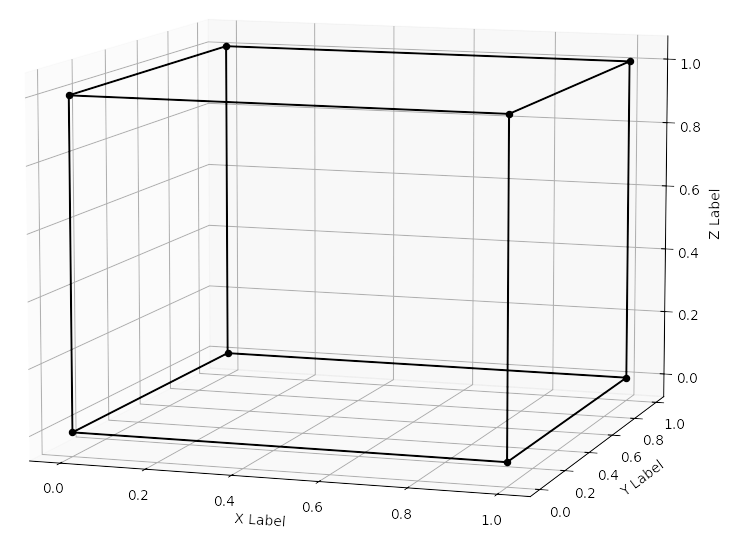
\includegraphics[width=0.7\linewidth]{images/ExampleCube.png}
	\caption{Расчетная область для кубика}
	\label{fig:ExampleCube}
\end{figure}

Попробуем подробить расчётную область (\ref{fig:ExampleCube}) на несколько частей. Получим сетку изображённую на рисунке (\ref{fig:GridCube}).

\begin{figure}
	\centering
	\vspace*{0.7cm}
	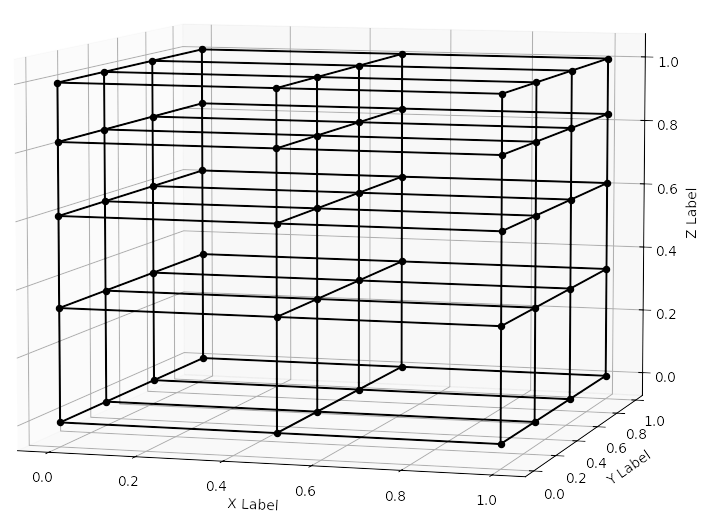
\includegraphics[width=0.7\linewidth]{images/GridCube.png}
	\caption{Секта для кубика}
	\label{fig:GridCube}
\end{figure}

Приведём ещё насколько примеров для построения сеток на шестигранниках, изображённых на рисунках  \ref{fig:Emerald} - \ref{fig:DEmerald}.

\begin{figure}
	\begin{minipage}[h]{0.49\linewidth}
		\center{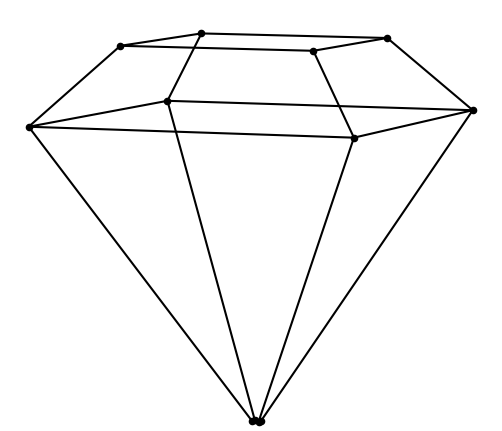
\includegraphics[width=0.5\linewidth]{images/EmeraldField.png} \\ а)}
	\end{minipage}
	\hfill
	\begin{minipage}[h]{0.49\linewidth}
		\center{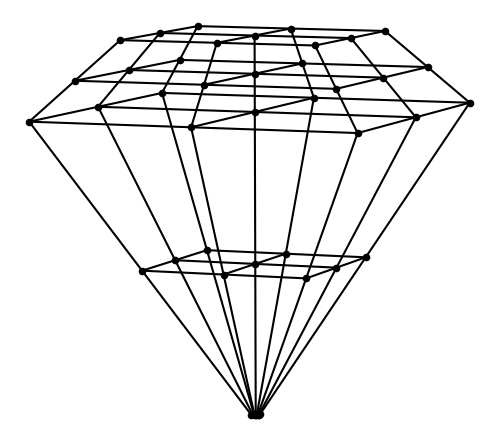
\includegraphics[width=0.5\linewidth]{images/EmeraldMesh.png} \\ б)}
	\end{minipage}
	\caption{Расчётная область в форме изумруда (а) и сетка к ней (б).}
	\label{fig:Emerald}
\end{figure}

\begin{figure}
	\begin{minipage}[h]{0.49\linewidth}
		\center{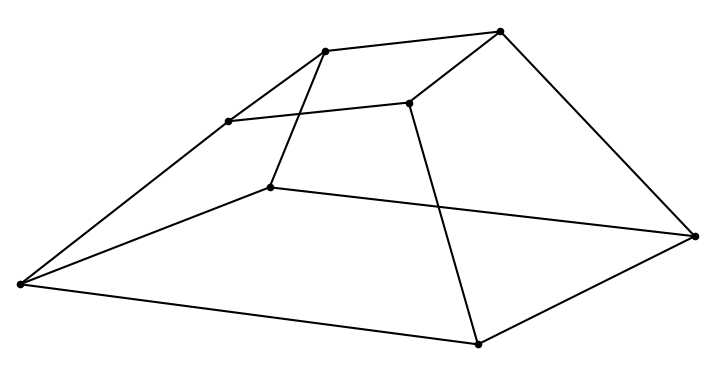
\includegraphics[width=0.5\linewidth]{images/PyramidField.png} \\ а)}
	\end{minipage}
	\hfill
	\begin{minipage}[h]{0.49\linewidth}
		\center{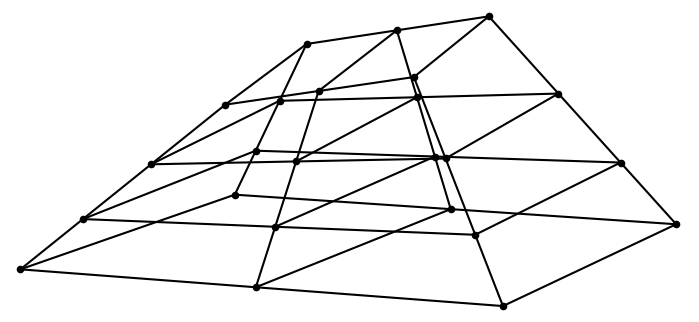
\includegraphics[width=0.5\linewidth]{images/PyramidMesh.png} \\ б)}
	\end{minipage}
	\caption{Расчётная область в форме скошенной пирамиды (а) и сетка к ней (б).}
	\label{fig:Pyramid}
\end{figure}

\begin{figure}
	\begin{minipage}[h]{0.49\linewidth}
		\center{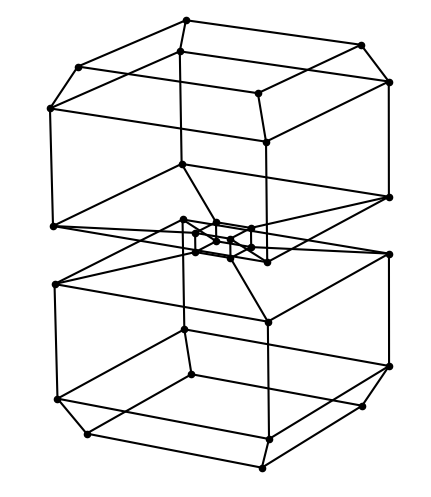
\includegraphics[width=0.5\linewidth]{images/HGField.png} \\ а)}
	\end{minipage}
	\hfill
	\begin{minipage}[h]{0.49\linewidth}
		\center{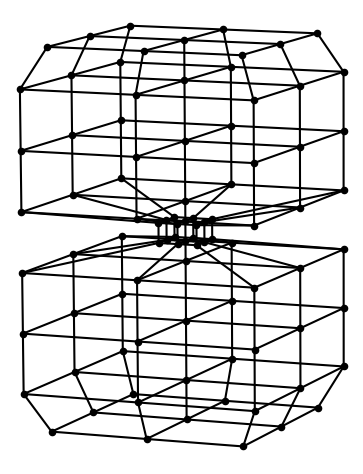
\includegraphics[width=0.5\linewidth]{images/HGMesh.png} \\ б)}
	\end{minipage}
	\caption{Расчётная область в форме песочных часов (а) и сетка к ней (б).}
	\label{fig:HG}
\end{figure}

\begin{figure}
	\begin{minipage}[h]{0.49\linewidth}
		\center{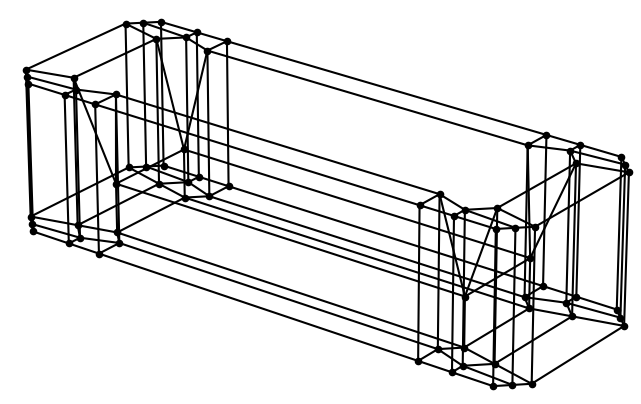
\includegraphics[width=0.5\linewidth]{images/BathField.png} \\ а)}
	\end{minipage}
	\hfill
	\begin{minipage}[h]{0.49\linewidth}
		\center{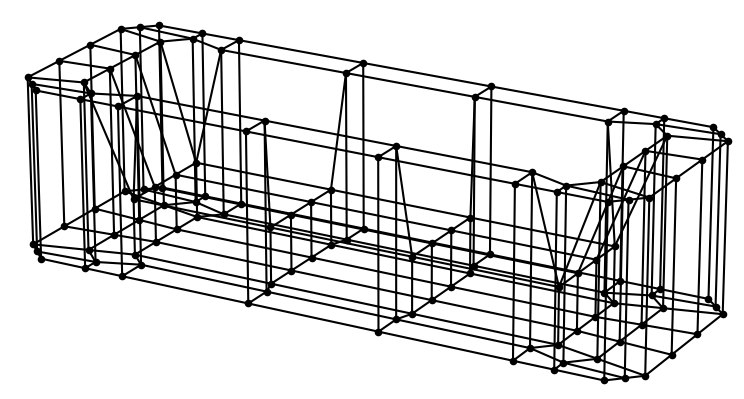
\includegraphics[width=0.5\linewidth]{images/BathMesh.png} \\ б)}
	\end{minipage}
	\caption{Расчётная область в форме ванной (а) и сетка к ней (б).}
	\label{fig:Bath}
\end{figure}

\begin{figure}
	\begin{minipage}[h]{0.49\linewidth}
		\center{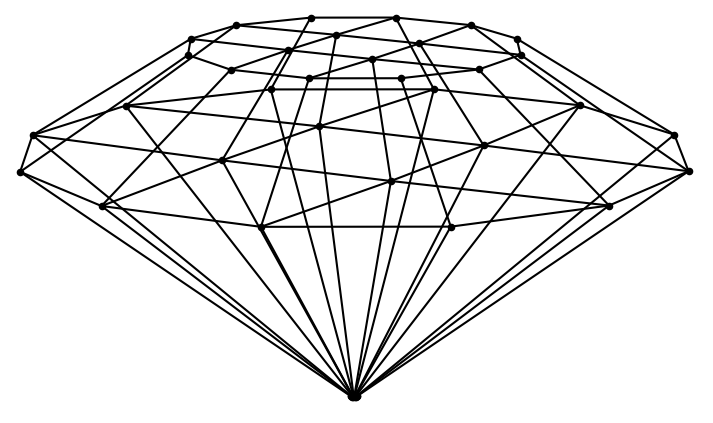
\includegraphics[width=0.5\linewidth]{images/DEmeraldField.png} \\ а)}
	\end{minipage}
	\hfill
	\begin{minipage}[h]{0.49\linewidth}
		\center{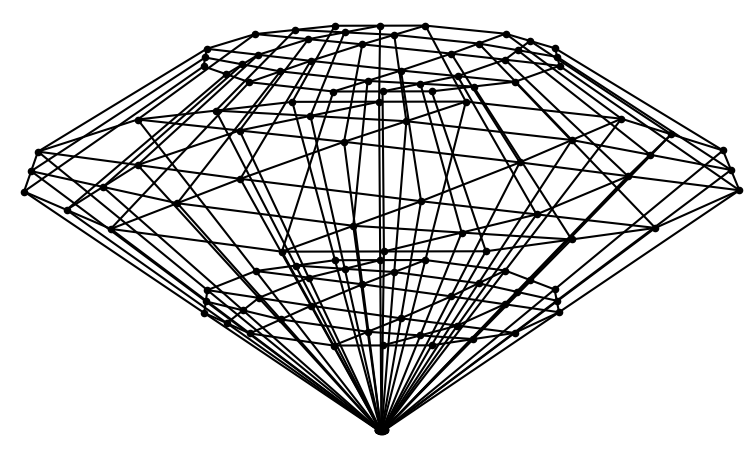
\includegraphics[width=0.5\linewidth]{images/DEmeraldMesh.png} \\ б)}
	\end{minipage}
	\caption{Расчётная область в форме детализированного изумруда (а) и сетка к ней (б).}
	\label{fig:DEmerald}
\end{figure}

Таким образом, программа для построения сетки может строить достаточно геометрически сложные фигуры.

\section{Численное интегрирование}

При расчёте элементов локальных матриц жёсткости (\ref{eq_1_11}) и масс (\ref{eq_1_12}) будем использовать численное интегрирование методами Гаусса разных порядков (2, 3, 4, 5). Результаты численного интегрирования на некоторых функциях приведены в таблицах \ref{tab:numIntegr1} - \ref{tab:numIntegr7}. Область интегрирования для всех функций единый: $\Omega_E \in \left[-1; 1\right]_x \cross \left[-1; 1\right]_y \cross \left[-1; 1\right]_z$.

\begin{table}
	\caption{Тестирование численного интегрирования на функции $u = 2$.}
	\centering
	\small
	\begin{tabularx}{1.0\textwidth}{| >{\raggedright\arraybackslash}X | >{\raggedright\arraybackslash}X | >{\raggedright\arraybackslash}X |>{\raggedright\arraybackslash}X |>{\raggedright\arraybackslash}X |}
		\hline
		\centering{Аналитический результат} & \centering{Гаусс 2} & \centering{Гаусс 3} & \centering{Гаусс 4} & \centering{Гаусс 5} \tabularnewline \hline
		
		\centering{16.0} & \centering{1.6000000e+01}& \centering{1.6000000e+01} & \centering{1.6000000e+01} & \centering{1.6000000e+01} \tabularnewline \hline
		
	\end{tabularx}
	\label{tab:numIntegr1}
\end{table}


\begin{table}
	\caption{Тестирование численного интегрирования на функции $u = x + y + z$.}
	\centering
	\small
	\begin{tabularx}{1.0\textwidth}{| >{\raggedright\arraybackslash}X | >{\raggedright\arraybackslash}X | >{\raggedright\arraybackslash}X |>{\raggedright\arraybackslash}X |>{\raggedright\arraybackslash}X |}
		\hline
		\centering{Аналитический результат} & \centering{Гаусс 2} & \centering{Гаусс 3} & \centering{Гаусс 4} & \centering{Гаусс 5} \tabularnewline \hline
		
		\centering{0.0} & \centering{0.0000000e+00}& \centering{-2.2204460e-16} & \centering{5.6898930e-16} & \centering{-6.5225603e-16} \tabularnewline \hline
		
	\end{tabularx}
	\label{tab:numIntegr2}
\end{table}

\begin{table}
	\caption{Тестирование численного интегрирования на функции $u = x^2 + y^2 + z^2$.}
	\centering
	\small
	\begin{tabularx}{1.0\textwidth}{| >{\raggedright\arraybackslash}X | >{\raggedright\arraybackslash}X | >{\raggedright\arraybackslash}X |>{\raggedright\arraybackslash}X |>{\raggedright\arraybackslash}X |}
		\hline
		\centering{Аналитический результат} & \centering{Гаусс 2} & \centering{Гаусс 3} & \centering{Гаусс 4} & \centering{Гаусс 5} \tabularnewline \hline
		
		\centering{8.0} & \centering{8.0000000e+00}& \centering{8.0000000e+00} & \centering{8.0000000e+00} & \centering{8.0000000e+00} \tabularnewline \hline
		
	\end{tabularx}
	\label{tab:numIntegr3}
\end{table}

\begin{table}
	\caption{Тестирование численного интегрирования на функции $u = x \cdot y \cdot z$.}
	\centering
	\small
	\begin{tabularx}{1.0\textwidth}{| >{\raggedright\arraybackslash}X | >{\raggedright\arraybackslash}X | >{\raggedright\arraybackslash}X |>{\raggedright\arraybackslash}X |>{\raggedright\arraybackslash}X |}
		\hline
		\centering{Аналитический результат} & \centering{Гаусс 2} & \centering{Гаусс 3} & \centering{Гаусс 4} & \centering{Гаусс 5} \tabularnewline \hline
		
		\centering{0.0} & \centering{8.0000000e+00}& \centering{0.0000000e+00} & \centering{0.0000000e+00} & \centering{8.6736174e-18} \tabularnewline \hline
		
	\end{tabularx}
	\label{tab:numIntegr4}
\end{table}

\begin{table}
	\caption{Тестирование численного интегрирования на функции $u = x^2 \cdot y^2 \cdot z^2$.}
	\centering
	\small
	\begin{tabularx}{1.0\textwidth}{| >{\raggedright\arraybackslash}X | >{\raggedright\arraybackslash}X | >{\raggedright\arraybackslash}X |>{\raggedright\arraybackslash}X |>{\raggedright\arraybackslash}X |}
		\hline
		\centering{Аналитический результат} & \centering{Гаусс 2} & \centering{Гаусс 3} & \centering{Гаусс 4} & \centering{Гаусс 5} \tabularnewline \hline
		
		\centering{$\frac{8}{27}$ $\approx$ 0.29630} & \centering{2.9629630e-01}& \centering{2.9629630e-01} & \centering{2.9629630e-01} & \centering{2.9629630e-01} \tabularnewline \hline
		
	\end{tabularx}
	\label{tab:numIntegr5}
\end{table}

\begin{table}
	\caption{Тестирование численного интегрирования на функции $u = \text{cos}(x + y + z)$.}
	\centering
	\small
	\begin{tabularx}{1.0\textwidth}{| >{\raggedright\arraybackslash}X | >{\raggedright\arraybackslash}X | >{\raggedright\arraybackslash}X |>{\raggedright\arraybackslash}X |>{\raggedright\arraybackslash}X |}
		\hline
		\centering{Аналитический результат} & \centering{Гаусс 2} & \centering{Гаусс 3} & \centering{Гаусс 4} & \centering{Гаусс 5} \tabularnewline \hline
		
		\centering{4.7666...} & \centering{4.7063579e+00}& \centering{4.7671091e+00} & \centering{4.7665835e+00} & \centering{4.7665859e+00} \tabularnewline \hline
		
	\end{tabularx}
	\label{tab:numIntegr6}
\end{table}

\begin{table}
	\caption{Тестирование численного интегрирования на функции $u = e^{x + y + z}$.}
	\centering
	\small
	\begin{tabularx}{1.0\textwidth}{| >{\raggedright\arraybackslash}X | >{\raggedright\arraybackslash}X | >{\raggedright\arraybackslash}X |>{\raggedright\arraybackslash}X |>{\raggedright\arraybackslash}X |}
		\hline
		\centering{Аналитический результат} & \centering{Гаусс 2} & \centering{Гаусс 3} & \centering{Гаусс 4} & \centering{Гаусс 5} \tabularnewline \hline
		
		\centering{12.9845...} & \centering{1.2857243e+01}& \centering{1.2983458e+01} & \centering{1.2984538e+01} & \centering{1.2984543e+01} \tabularnewline \hline
		
	\end{tabularx}
	\label{tab:numIntegr7}
\end{table}

\section{Процесс построения локальных матриц жёсткости и масс}

Рассмотрим процесс построения локальных матриц жёсткости и масс. При генерации локальной матрицы масс на параллелепипеде в векторном МКЭ используется следующая локальная матрица

\begin{equation} \label{eq_2_1}
	\begin{gathered}
		\hat{\textbf{M}} = \gamma \frac{h_x h_y h_z}{36} 
		\begin{pmatrix} 
			\textbf{D} & \textbf{0} & \textbf{0}\\
			\textbf{0} & \textbf{D} & \textbf{0}\\
			\textbf{0} & \textbf{0} & \textbf{D}\\
		\end{pmatrix},
	\end{gathered}
\end{equation}
где $\textbf{0}$ - матрица размером 4 $\cross$ 4, полностью заполненная нулями, а

\begin{equation*}
	\begin{gathered}
		\hat{\textbf{D}} =
		\begin{pmatrix}
			4 & 2 & 2 & 1\\
			2 & 4 & 1 & 2\\
			2 & 1 & 4 & 2\\
			1 & 2 & 2 & 4\\
		\end{pmatrix}.
	\end{gathered}
\end{equation*}

Тогда на единичном элементе $\Omega_E \in \left[-1; 1\right]_x \cross \left[-1; 1\right]_y \cross \left[-1; 1\right]_z$ и при $\gamma = 1$ матрица (\ref{eq_2_1}) примет вид:


\begin{equation*}
	\begin{gathered}
		\hat{\textbf{M}} = \frac{2}{9} 
		\begin{pmatrix} 
			\textbf{D} & \textbf{0} & \textbf{0}\\
			\textbf{0} & \textbf{D} & \textbf{0}\\
			\textbf{0} & \textbf{0} & \textbf{D}\\
		\end{pmatrix}.
	\end{gathered}
\end{equation*}

Попробуем сделать ту же самую процедуру при $\gamma = 1$ и на элемента $\Omega_E \in \left[-1; 1\right]_x \cross \left[-1; 1\right]_y \cross \left[-1; 1\right]_z$, но используя интегралы из (\ref{eq_1_12}). Элементы сгенерированной матрицы в виде консольного вывода программы изображены на рисунке \ref{fig:GeneratedMatrixMass}.

\begin{figure}
	\centering
	\vspace*{0.7cm}
	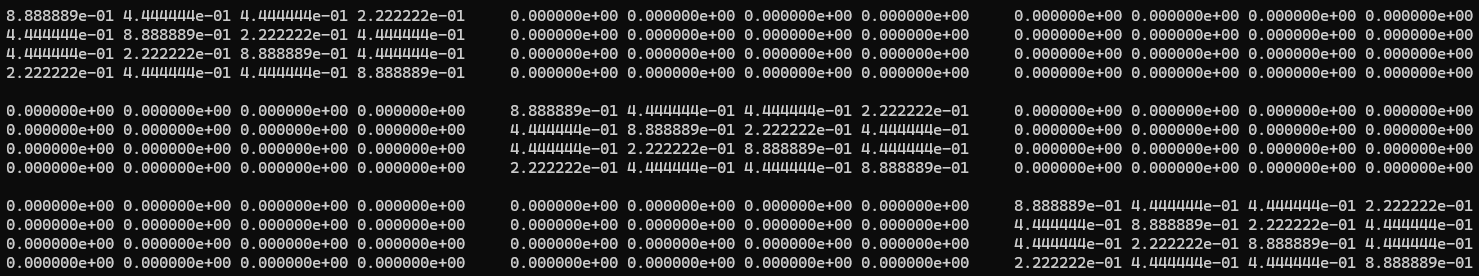
\includegraphics[width=1.0\linewidth]{images/M.png}
	\caption{Консольный вывод сгенерированной матрицы масс на $\Omega_E$}
	\label{fig:GeneratedMatrixMass}
\end{figure}

Локальная матрица жёсткости $\hat{\textbf{G}}$ на параллелепипеде $\Omega_E \in \left[-1, 1\right]_x \cross \left[-1, 1\right]_y \cross \left[-1, 1\right]_z$ при $\overline{\mu} = 1$ принимает вид:

\begin{equation*}
	\hat{\textbf{G}} = \left(
	\begin{array}{ccc}
		\frac{1}{3}\textbf{G}_1 + \frac{1}{3}\textbf{G}_2 & -\frac{1}{3}\textbf{G}_2 & \frac{1}{3}\textbf{G}_3 \\
		-\frac{1}{3}\textbf{G}_2 & \frac{1}{3}\textbf{G}_1 + \frac{1}{3}\textbf{G}_2 & -\frac{1}{3}\textbf{G}_1 \\
		\frac{1}{3}\textbf{G}^\text{T}_3 & -\frac{1}{3}\textbf{G}_1 & \frac{1}{3}\textbf{G}_1 + \frac{1}{3}\textbf{G}_2 \\
	\end{array}
	\right),
\end{equation*}
где
\begin{equation*}
	\textbf{G}_1 = \left(
	\begin{array}{rrrr}
		2 & 1 & -2 & -1 \\
		1 & 2 & -1 & -2 \\
		-2 & -1 & 2 & 1 \\
		-1 & -2 & 1 & 2 \\
	\end{array}
	\right),
	\hspace{10mm}
	\textbf{G}_2 = \left(
	\begin{array}{rrrr}
		2 & -2 & 1 & -1 \\
		-2 & 2 & -1 & 2 \\
		1 & -1 & 2 & -2 \\
		-1 & 1 & -2 & 2 \\
	\end{array}
	\right),
\end{equation*}

\begin{equation*}
	\textbf{G}_3 = \left(
	\begin{array}{rrrr}
		-2 & 2 & -1 & 1 \\
		-1 & 1 & -2 & 2 \\
		2 & -2 & 1 & -1 \\
		1 & -1 & 2 & -2 \\
	\end{array}
	\right).
\end{equation*}

Теперь, проверим генерацию матрицы жёсткости через формулу (\ref{eq_1_11}). Консольный вывод содержимого матрицы указан на рисунке \ref{fig:GeneratedMatrixStiffness}

\begin{figure}
	\centering
	\vspace*{0.7cm}
	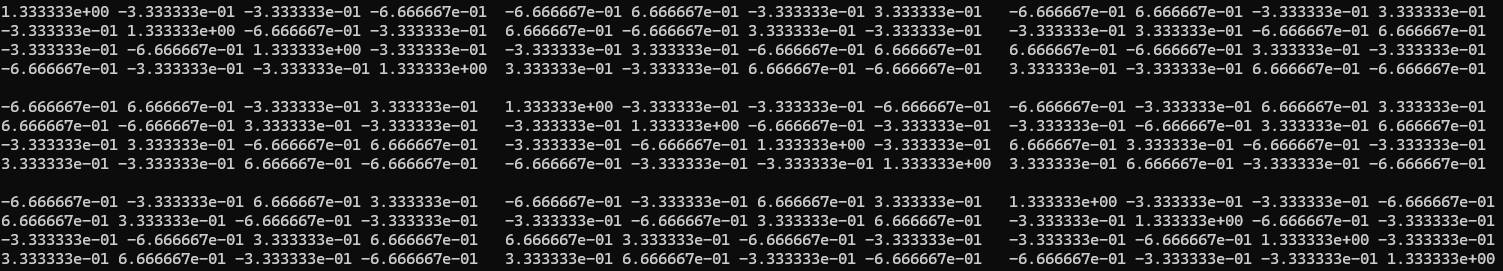
\includegraphics[width=1.0\linewidth]{images/G.png}
	\caption{Консольный вывод сгенерированной матрицы масс на $\Omega_E$}
	\label{fig:GeneratedMatrixStiffness}
\end{figure}

\section{Решение СЛАУ}

Через LOS или Pardiso.





%\textbf{Здесь будет программная реализация $\downarrow$}

